%%
%% This is file `mcmthesis-demo.tex',
%% generated with the docstrip utility.
%%
%% The original source files were:
%%
%% mcmthesis.dtx  (with options: `demo')
%% 
%% -----------------------------------
%% 
%% This is a generated file.
%% 
%% Copyright (C)
%%     2010 -- 2015 by Zhaoli Wang
%%     2014 -- 2016 by Liam Huang
%% 
%% This work may be distributed and/or modified under the
%% conditions of the LaTeX Project Public License, either version 1.3
%% of this license or (at your option) any later version.
%% The latest version of this license is in
%%   http://www.latex-project.org/lppl.txt
%% and version 1.3 or later is part of all distributions of LaTeX
%% version 2005/12/01 or later.
%% 
%% This work has the LPPL maintenance status `maintained'.
%% 
%% The Current Maintainer of this work is Liam Huang.
%% 
\documentclass{mcmthesis}
\mcmsetup{CTeX = false,   % 使用 CTeX 套装时,设置为 true
        tcn = 1902081, problem = C,
        sheet = true, titleinsheet = true, keywordsinsheet = true,
        titlepage = false, abstract = true}
\usepackage{palatino}
\usepackage{lipsum}
\usepackage{indentfirst}
\usepackage{booktabs}
\setlength{\parindent}{2em}
\title{Title}
\author{\small \href{http://www.latexstudio.net/}
  {
\includegraphics[width=7cm]{mcmthesis-logo}}}
\date{\today}
\begin{document}
\begin{abstract}
%\lipsum[1]
\begin{keywords}
keyword1; keyword2
\end{keywords}
\end{abstract}
\maketitle

\tableofcontents

\newpage

\section{Introduction}



\section{CA Model}

To consider the relationship between adjacent counties, CA Model is introduced. Due to the specificity of this problem, we will modify the traditional CA Model to satisfy the limitations of this problem. \par


\subsection{Properties} % or maybe description

CA Model is consisted of multiple cells with state and the relartionship of adjacence. Here we present several properties regarding our revised CA Model. 

\begin{itemize}
\item In our revised CA Model, a cell represents some county in the five states.
\item The state of a cell denotes the number of predicted drug reports of some county.
\item Any two cells are adjecent in CA Model if and only if the two counties they respectively represent are geographically adjecnt.
\item In a new stage, some cell's state is determined by this cell's state and its neighbours' state in the previous stage.
\end{itemize}

Our revised CA Model differs from traditional CA Model in several aspects. 
\begin{enumerate}
\item \textbf{Number of  states}.\\
As the state of cell is equivalent to the number of some county's drug reports, the cell in our revised CA Model has infinite kinds of state. However, the cell in traditional CA Model are restricted to finite kinds of state.
\item \textbf{Number of neighbours}\\
Traditional CA model has to restrict the number of neighbours to be 4 or 8. In our CA Model, we shed the constraint by using arrays to store the neighbours, which implies that we can have theoretically infinite neighbours.
\end{enumerate}

\begin{figure}[h]
\small
\centering
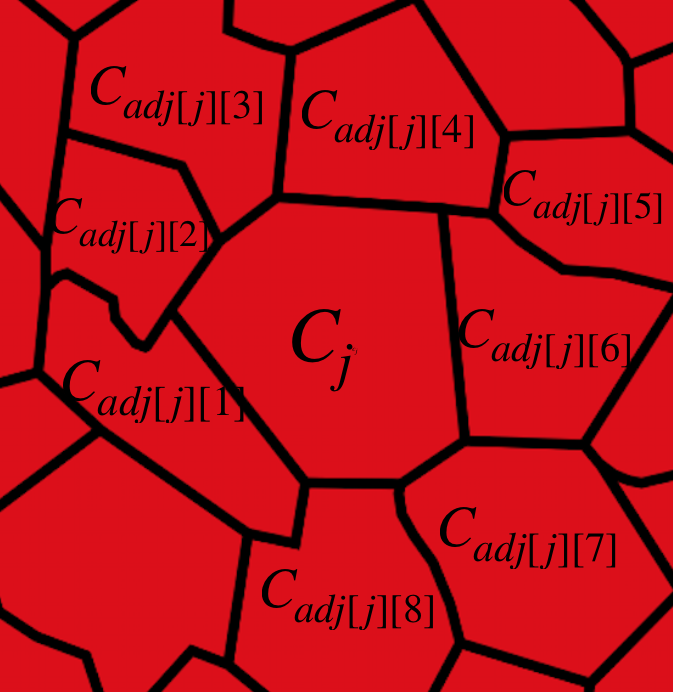
\includegraphics[width=8cm]{CA_rules.png}
\caption{neighbours} \label{fig:neighbours}
\end{figure}


\subsection{Symbols}


\begin{table}[!h]
\centering
\caption{Main Symbols used in CA Model} %\label{tab:aStrangeTable}
\begin{tabular}{ll}
\toprule[2.5pt]
\textbf{Symbols}& \textbf{Definition} \\
\midrule[1.5pt]
$c_j$ & the $j_{th}$ cell \\
\midrule
$s_{ij}$& the $j_{th}$ cell's state in stage $i$ \\
\midrule
$s_{ij}'$& the $j_{th}$ cell's state in stage $i$ (only for backstepping)\\
\midrule
$r_{ij}$ & the $j_{th}$ cell's real data in stage $i$ \\
\midrule
$n_{j}$ & the number of the $j_{th}$ cell's neighbours\\
\midrule
$adj[j]$ & the array which stores the $j_{th}$ cell's neighbours \\
 & We can use $adj[j][k]$ to index the neighbours of the cell, where $k = 1,...,n_{j}$\\
\midrule
$N$ & the number of counties in the five States\\
\midrule
$\lambda$ & a constant which describes the degree of adjecnt counties's contact \\
\bottomrule
\end{tabular}
\end{table}


\newpage
\subsection{Prediction Rules }
Any cell's state in the $(i+1)_{th}$ stage is determined by its state and its neighbours' state in the $i_{th}$ stage. In other words, $s_{(i+1)j}$ is determined by $s_{ij}$ and $s_{ik}$ where $c_k$ is a neighour of $c_j$.\par
With careful consideration, We choose the relationship to be linear. The Prediction formula is as follows.
      $$ s_{(i+1)j} \ = \ k_1 s_{ij} \ + \ k_2 \lambda \frac{\sum\limits_{k=1} ^{n_j} s_{i (adj[j][k])} }{n_j} $$
    where $k_1$ denotes the influence of its own state, $k_2$ denotes the infulence of its neighbours' state, $\lambda$ is a constant which describes the degree of adjecnt counties's contact. After multiple tests and the consideration of reality, we choose $\lambda$ to be 0.3.\par

    This Prediction formula takes both the cell's influence and its neighbours' influence into consideraion.
\subsection{Backstepping Rules}
    We also need to estimate the data in years before 2010 which is not provided. We simply rewrite the formulation above and make some approximation. To distinguish Prediction formula, we use $s_{ij}'$ to replace $s_{ij}$. The formula is as follows:

       $$ s_{ij}' = \frac{s_{(i+1)j}'}{k_1} - \frac{k_2}{k_1} \lambda \frac{\sum\limits_{k=1} ^{n_j} s_{(i+1) adj[j][k]}' }{n_j} $$
      
      where $k_1$ , $k_2$ and $\lambda$ are identical to those in Prediction Rules. 

\subsection{Determine coefficients} \label{Section:Determine coefficients}
    To determine the coefficients $k_1$ and $k_2$, we use program to help us choose between $0$ and $1$ automatically. We have data about drug reports in years 2010-2017. The program will choose between $0$ and $1$ by step $0.001$  to minimize the error. The formula to calculate error is as follows.
    $$error = \frac{\sum\limits_{i=2011}^{2017} \sum_{j=1}^{N} (r_{ij} - s_{ij})^2  }{N * (2017-2011+1)}$$ 
    where $N$ is the number of counties in the five state. \par
    Given $\lambda=0.3$, we find the error is minimal when $k_1=0.999$ and $k_2=0.186$. Based on this, we can conclude that the cell's own influence is of most significance, but the influence of adjacent cells cannot be ignored.

\subsection{Appliance of the CA Model}

\begin{figure}[h]
\small
\centering
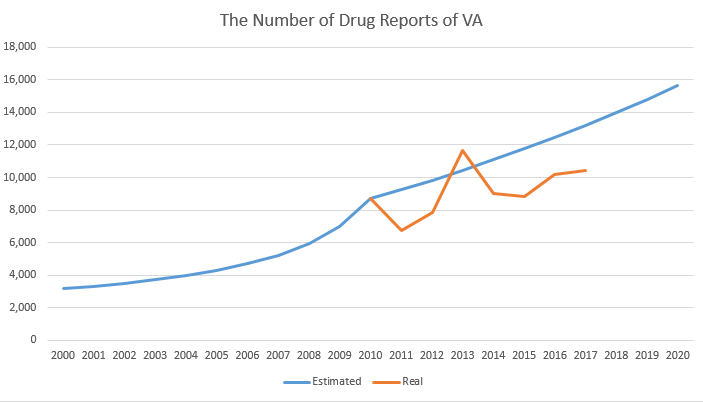
\includegraphics[width=12cm]{CA_of_VA.png}
\caption{The number of drug reports of VA} \label{fig:CA_of_VA}
\end{figure}

\begin{figure}[h]
\small
\centering
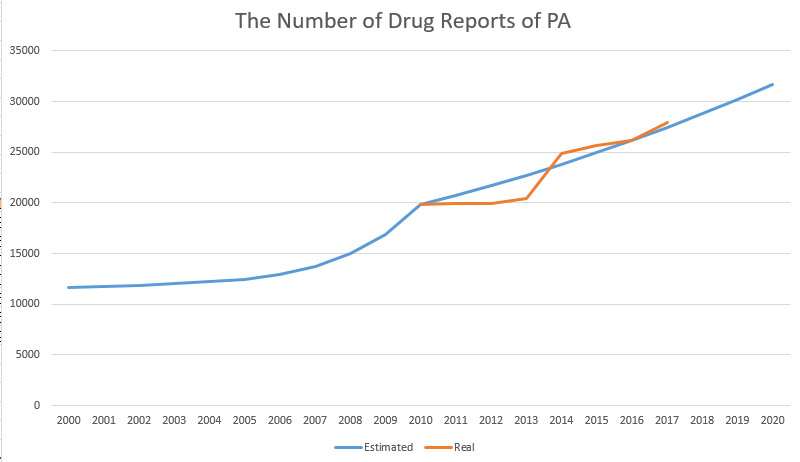
\includegraphics[width=12cm]{CA_of_PA.png}
\caption{The number of drug reports of PA} \label{fig:CA_of_PA}
\end{figure}

  We have estimated the number of drug reports of every county in years from 2000 to 2030 using our revised CA model. Therefore we can estimate the data of every state by summing the data of its counties. Fig.\ref{fig:CA_of_VA} shows the estimated data and real data of VA. And Fig.\ref{fig:CA_of_PA} shows the estimated data and real data of PA. CA Model fits well with the State PA, where two lines are very close. As to the State VA, two lines have similar trends.\par
  Using CA Model, we can get data of counties, which means we can get geographical distribution of data. This may provide insight into the data. 
\begin{figure}[h]
\small
\centering
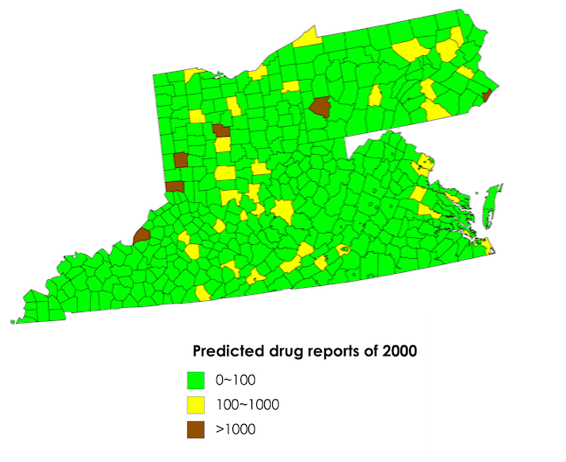
\includegraphics[width=12cm]{CA_2000.png}
\caption{Estimated Geographical Distribution in the year 2000} \label{fig:CA_2000}
\end{figure}

\begin{figure}[h]
\small
\centering
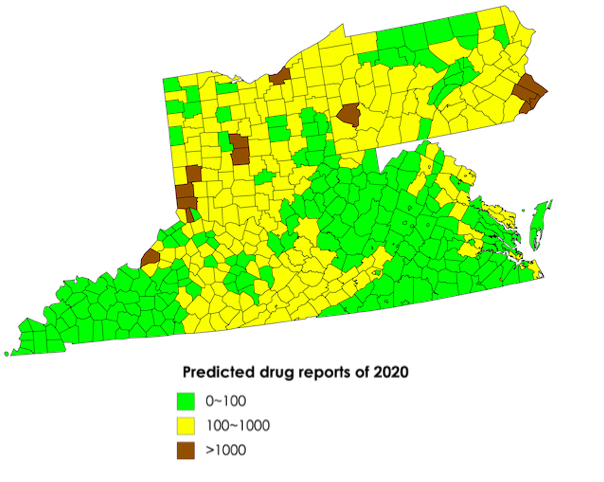
\includegraphics[width=12cm]{CA_2020.png}
\caption{Estimated Geographical Distribution in the year 2020} \label{fig:CA_2020}
\end{figure}

In Fig.\ref{fig:CA_2000}, there are six counties with estimated numbers greater than $1000$ in the year 2000, namely Delware(OH)  , Jefferson(KY), Montgomery(OH), Allegheny(PA), Hamilton(OH), Philadelphia(PA). In Fig.\ref{fig:CA_2020}, there are thirteen counties with estimated numbers greater than $1000$ in the year 2020. We can notice that the growth in number spread from the red regions in Fig.\ref{fig:CA_2000}。 Therefore we may conclude that the drug abuse might have started form the red regions in Fig.\ref{fig:CA_2000}.


\subsection{Sensitivity Analysis}
  As the constant $\lambda$ in CA Model may be hard to obtain or there might be some uncertainty, the choice of $\lambda$ might affect the result of our CA Model. So in order to test the robustness of our revised CA Model , a sensitivity analysis is conducted by testing our CA Model with various $\lambda$. \par
  Here we calculate the error by the formula in Section \ref{Section:Determine coefficients}. We originally choose $\lambda=0.3$. To test the robustness of our CA Model, we set $\lambda=0.5$ and $0.8$ respectively. The tests showed that our model is robust.

  \begin{table}[!h]
\centering
\caption{The influence of $\lambda$'s change on error} %\label{tab:aStrangeTable}
\begin{tabular}{ccc|c}
\toprule[2.5pt]
$\lambda$ & $k_1$ & $k_2$ & error \\
\midrule[1.5pt]
0.3 \ \ \ \ &  \ \ \ \ 0.999 \ \ \ \ & \ \ \ \ 0.186 \ \ \ \ & \ \ \ \ 78691.4 \\
\midrule
0.5 \ & \ 0.999 \ & \ 0.112 \ & \ 78694.1 \\
\midrule
0.8 \ & \ 0.999 \ & \ 0.070 \ & \ 78694.1 \\
\bottomrule
\end{tabular}
\end{table}


\begin{thebibliography}{99}

\end{thebibliography}

\begin{appendices}


\end{appendices}
\end{document}

%% 
%% This work consists of these files mcmthesis.dtx,
%%                                   figures/ and
%%                                   code/,
%% and the derived files             mcmthesis.cls,
%%                                   mcmthesis-demo.tex,
%%                                   README,
%%                                   LICENSE,
%%                                   mcmthesis.pdf and
%%                                   mcmthesis-demo.pdf.
%%
%% End of file `mcmthesis-demo.tex'.
